\chapter{Problem Context: UE Context Management and Predictability\label{chapter:context}}
\chaptermark{Problem Context}

\section{The UE Context Management subsystem}\label{sec:uecm}
The subsystem under study is a UE Context Management service, modelled on a real Nokia
gNB-CU-CP service domain that owns the UE context lifecycle, RRC procedure
execution~\cite{3gpp38331}, and mobility/handover, the functions the 3GPP architecture assigns
to the control-plane part of a disaggregated gNB (Section~\ref{sec:ranarch}).
Figure~\ref{fig:fsm} shows the UE-context lifecycle state machine both implementations encode
identically and the mixed workload of Section~\ref{sec:workload} walks each UE through.

\begin{figure}[ht]
\centering
\begin{tikzpicture}[
    ->, >=Stealth, node distance=3.2cm, font=\small,
    every state/.style={draw, minimum size=1.5cm, fill=blue!6, thick},
    every edge/.style={draw, thick}
  ]
  \node[state, initial, initial text=\scriptsize create] (idle) {Idle};
  \node[state, right=of idle] (conn) {Connected};
  \node[state, right=of conn] (reconf) {Reconf.};
  \node[state, below=1.9cm of conn, fill=gray!10] (rel) {Released};

  \path (idle)  edge node[above,font=\scriptsize]{setup} (conn)
        (conn)  edge[bend left=18] node[above,font=\scriptsize]{begin} (reconf)
        (reconf) edge[bend left=18] node[below,font=\scriptsize]{complete / abort} (conn)
        (conn)  edge node[right,font=\scriptsize,pos=0.45]{release} (rel)
        (idle)  edge[bend right=32] node[below,font=\scriptsize,pos=0.6]{release} (rel);
  \path (conn) edge[loop above] node[font=\scriptsize]{signal / add\_drb} (conn);
\end{tikzpicture}
\caption[UE-context lifecycle state machine]{UE-context lifecycle state machine. \texttt{create} allocates a context in
\texttt{Idle}, \texttt{setup} connects it, and \texttt{signal} and \texttt{add\_drb} are handled
in place while \texttt{Connected}. Operations invalid for the current state return an
\texttt{OpError} instead of changing state.\label{fig:fsm}}
\end{figure}

\paragraph{Why this subsystem.}
UECM is core RAN layer-3 functionality carrying the properties that make production
control-plane code difficult: per-UE mutable state, a strict operation lifecycle, high
concurrency across UEs, and the latency and reliability targets the 5G system sets for
control-plane procedures~\cite{3gpp38913,3gpp22261}. Conclusions about how a language handles
those properties therefore transfer to other stateful, concurrent control-plane services. It is
also small enough to specify precisely, implement faithfully in two languages, and reason about
in full, which is what makes a parity-tested comparison possible. A larger subsystem would buy
external validity at the cost of the internal validity a fair language comparison depends on.

\paragraph{Operation set.}
The interface exercised by the study is deliberately small and lifecycle-oriented: create and
release a context, set up a connection (\texttt{Idle}$\rightarrow$\texttt{Connected}), handle an
in-session signalling message, add a data radio bearer, begin, complete, or abort a
reconfiguration or handover, and look up a context's state under concurrent load. Every
operation is defined for every state of Figure~\ref{fig:fsm}, and one illegal in the current
state returns a typed error and leaves the context unchanged rather than throwing or corrupting
state. That closed, well-typed set lets the same test vectors and the same workload drive both
implementations along identical paths (Section~\ref{sec:parity}).

\section{Memory-safety and concurrency defect classes}\label{sec:defects}
The defects that affect C++ control-plane code of this kind fall into two families. The
\emph{memory-safety} family concerns the lifetime and bounds of objects: a \emph{use-after-free}
accesses already released storage, a \emph{double-free} releases the same storage twice, and a
\emph{buffer overflow} reads or writes past the end of an allocation. The \emph{concurrency}
family concerns unsynchronised or ill-ordered access from multiple threads: a \emph{data race}
is a pair of unsynchronised accesses to one location of which at least one is a write, a
\emph{deadlock} is a cyclic wait for locks, and \emph{iterator invalidation} uses an iterator or
reference into a container after a mutation has moved or freed the underlying storage. All of
them are \emph{silent} in C++. Each is accepted by the compiler and may appear to work on the
paths ordinary tests happen to exercise, surfacing only later as corruption, a crash, or an
unpredictable latency spike. These are the same memory-corruption classes decades of security
research have struggled to contain in C and C++~\cite{szekeres2013sok}.

Table~\ref{tab:defectmap} gives each class the form it would plausibly take here, which is what
makes the subsystem a good vehicle for studying them. Two of the seven are carried for what the
C++ tooling does \emph{not} say about them. The use-after-move leaves the acknowledgement
carrying an empty identity, but nothing is corrupted and nothing is undefined, because a
moved-from object is in a valid but unspecified state, so no sanitiser has a runtime symptom to
find. The thread-unsafe handle's correctness constraint is written in a comment, because C++ has
no way to state thread affinity in a type.

These seven lie squarely within the guarantees Rust claims to provide, which makes them the
natural test of whether that claim holds. Testing only them would build the expected answer into
the choice of test cases, so seven further classes are carried into the study for the opposite
reason, because there is good reason to expect that safe Rust does \emph{not} prevent them, and
the reason differs by class. A lock-order deadlock violates nothing about object lifetimes or
aliasing. The fault is in the order of acquisition. The lost update is a \emph{race condition}
rather than a \emph{data race}, because the atomicity violation lives in the composition of the
two critical sections and not in the accesses themselves, each of which is synchronised.
Reference counting cannot collect a cycle in either language, and leaking is safe in Rust by
explicit design, so the reference-cycle leak is the catalogue's cleanest statement of a
boundary, with both languages failing identically. C++ signed overflow is \emph{undefined}, so a
bearer's overflowing tunnel endpoint identifier (TEID) stride computation has no meaning at all,
whereas Rust \emph{defines} it to wrap, because the \texttt{opt-level~=~2} profile this study
compares leaves \texttt{overflow-checks} off, so the program has a meaning and the meaning is
wrong. CVE-2026-64467 in \texttt{rust\_binder} is a stride error of that shape, so the pattern
is not hypothetical. The concurrency model of Section~\ref{sec:concurrency} makes a shard a
failure domain by construction, and neither type system enforces that it behaves as one: a C++
exception escaping the thread callable terminates the whole process, while a Rust panic is
confined to its thread but poisons the state it held, so the damage propagates along the data
instead. Carrier-grade availability rests on that domain holding. Double-free across the seam is
that same retransmitted release in the form a foreign-function boundary has to give it. Safe
Rust rejects it because ownership tracks the value, and a seam cannot keep that, since handing a
raw pointer to a C caller is the operation that ends the compiler's knowledge of it. The class
therefore appears on both sides of the boundary, which states most sharply what the boundary is.
Rust likewise removes the ordinary form of the forgotten lock guard, because a guard releases
when it is dropped and there is no hand-written unlock to skip, but not the bug, because a guard
is a value and leaking a value is safe. Where the reference cycle leaks memory, this leaks the
context itself.

Together these fourteen form the catalogue injected in Chapter~\ref{chapter:eval}, and the split
between the two groups is what lets the study report a boundary rather than a verdict. Buffer
overflow is described for completeness and not injected, because an injected instance would be
an artificial construct rather than a plausible bug here. The table records the outcome expected
of each case \emph{before} the study was run, which is the form the runner records it in,
because an expectation written down in advance can be violated in either direction and reported
as a discrepancy, whereas one formed after the fact cannot.

\begin{table}[H]
\centering
\small
\caption[The injected catalogue and its incarnations in UECM]{The injected defect catalogue: each class in the form it would plausibly take in UE
Context Management, and the outcome recorded for it in advance of the study. The last column
is a prediction rather than a result. Table~\ref{tab:taxonomy} reports what was measured, and
the fault runner flags a mismatch in either direction instead of absorbing it into the
conclusion. Buffer overflow is listed for completeness and not injected: neither
implementation does pointer arithmetic on the context store.\label{tab:defectmap}}
\footnotesize
\renewcommand{\arraystretch}{0.95}
\begin{tabular}{@{}R{0.19\linewidth} R{0.40\linewidth} R{0.14\linewidth} R{0.16\linewidth}@{}}
\hline\hline
Defect class & Incarnation in UE Context Management & How it fails & Expected in safe Rust \\
\hline
\multicolumn{4}{@{}l}{\emph{Memory-safety family: object lifetime and bounds}} \\
Use-after-free & An in-flight signalling handler dereferences a context that a concurrent \texttt{release} has already erased from the map & Corruption or crash & Prevented \\
Double-free & A retransmitted release is not made idempotent, so the release path frees the context's resources a second time & Corruption or crash & Prevented \\
Use-after-move & Admission answers the request from the context it has just moved into the store & Silently empty identity & Prevented \\
Buffer overflow & No plausible incarnation here: the context store is reached only through container APIs & n/a & Not injected \\
\hline
\multicolumn{4}{@{}l}{\emph{Concurrency family: unsynchronised or ill-ordered access}} \\
Iterator invalidation & A bearer is added while the context's data-radio-bearer list is being iterated & Corruption or crash & Prevented \\
Data race & Two workers update the same context field, a counter or a state flag, without synchronisation & Torn or lost value & Prevented \\
Unguarded shared mutation & A context is shared across threads and mutated with no ownership rule governing it & Torn or lost value & Prevented \\
Thread-unsafe handle shared & A context handle whose refcount is not atomic is passed to two shard workers & Corrupted refcount & Prevented \\
\hline
\multicolumn{4}{@{}l}{\emph{Boundary group: included because safe Rust is expected \emph{not} to prevent them}} \\
Lock-order deadlock & Opposing handovers lock source-then-target and target-then-source & Hang & Not prevented \\
Lost update & A counter's read-modify-write is split across two critical sections, so each access is synchronised but their composition is not atomic & Silently wrong value & Not prevented \\
Reference-cycle leak & A context and its handover peer hold owning references to each other, so neither reference count reaches zero & Unbounded growth & Not prevented \\
Integer overflow (release build) & A bearer's TEID stride computation exceeds the width of its type & Silently wrong value & Not prevented \\
Worker-failure blast radius & One shard worker fails part-way through a procedure while holding shard state & Outage beyond one shard & Not prevented \\
Double-free across the seam & A C++ host releases an opaque handle to a Rust context twice & Corruption or crash & Not prevented \\
Forgotten lock guard & Bearer setup returns on a validation failure without releasing the context lock & Hang & Not prevented \\
\hline
\end{tabular}
\end{table}

\section{Tail latency and predictability in RAN}
Section~\ref{sec:predictability} set out why the tail rather than the mean governs a
latency-critical system, and what measuring it correctly demands. Two properties of the RAN
setting turn that methodological preference into the governing metric, and
Figure~\ref{fig:tailconcept} draws them: fan-out and scale. One user-visible action, a call
setup or a handover, becomes many dependent control-plane operations whose slowest member gates
completion, and a busy site drives thousands of such procedures per second across millions of
connected devices. The p99.9 of a single UE Context Management operation is therefore not a
curiosity at the margin of a distribution but a rate of degraded procedures the network sustains
continuously.

That scale is not hypothetical. A measurement study of a disaggregated 5G RAN times the
CU-CP-to-DU UE Context Setup procedure over F1-C and the CU-CP-to-CU-UP bearer context setup
over E1 under different interface-protection schemes, and finds the choice worth hundreds of
microseconds: on F1-C, Internet Protocol Security (IPsec) adds on the order of $120\,\mu$s on
average to UE context setup, against roughly $430\,\mu$s for Datagram Transport Layer Security
(DTLS)~\cite{michaelides2026ranlatency}. Overheads of that size are treated as consequential for
precisely the procedure family this thesis reimplements, which places these operations in a
regime where tens of microseconds are an engineering quantity rather than noise.

The study therefore characterises the full latency distribution, focusing on the high
percentiles (p99, p99.9 and p99.99) and the maximum, and on how these degrade as offered load
approaches and then exceeds saturation (Chapter~\ref{chapter:eval}). Queueing delay grows
super-linearly near capacity, so stopping at nominal load would miss the regime that decides
service quality, and that regime is also where a difference between two implementations of one
design, if there is one, has room to become visible.

\begin{figure}[ht]
\centering
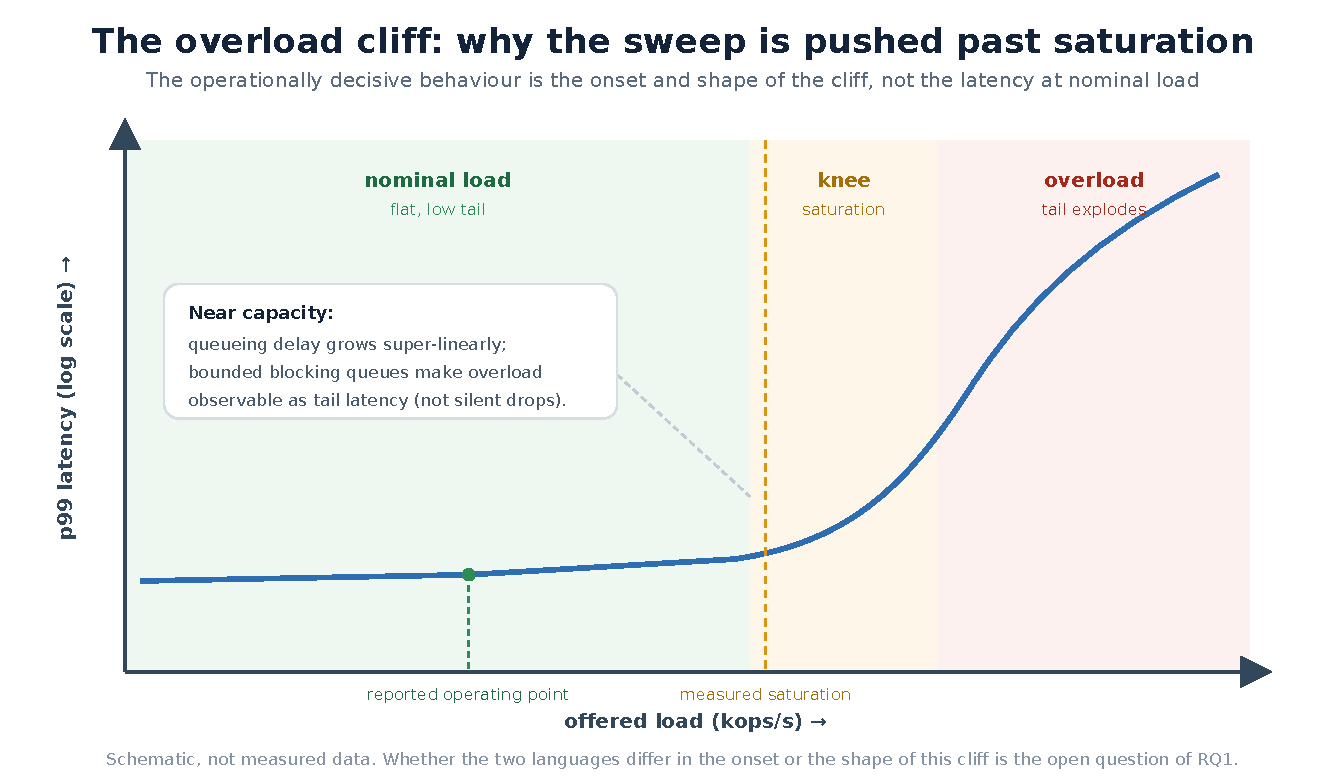
\includegraphics[width=0.70\linewidth]{diagrams/pdf/15_overload_cliff.pdf}
\caption[The overload cliff]{The overload cliff. Tail latency stays low and flat while offered load is below
service capacity, then climbs steeply once the system is driven past saturation and requests
queue behind the bounded, blocking queues. The operationally decisive behaviour is the onset and
shape of this cliff, which is why the load sweep is pushed beyond the saturation point rather
than stopping at nominal load. The figure is a schematic of the phenomenon and not a plot of
this study's data: Whether the two languages differ in where the cliff begins or in what they
sustain beyond it is exactly what RQ1 asks, and Sections~\ref{sec:perfresults}
and~\ref{sec:overload} report that they differ in both. How steeply the cliff rises is not compared
between them, for the reason Section~\ref{sec:stats} fixes in
advance.\label{fig:cliff}}
\end{figure}

